\batchmode
\documentclass{beamer}
\usepackage[utf8]{inputenc}
\usepackage[T1]{fontenc}
\usepackage[ngerman]{babel}
\usepackage{amsmath}

\usetheme[deutsch]{KIT}
\author{Jan Haag (jan.haag@student.kit.edu)}
\title{Programmieren Tutorium 12 -- Abschlussaufgabe, Teil 1}
\institute{Institut f\"{u}r Zeritfizierbare und Vertrauensw\"{u}rdige Informatiksysteme (ZVI)}
\TitleImage[scale=0.225]{frontpic.jpg}

\begin{document}
\begin{frame}
\maketitle
\end{frame}

\section{Aufgabe}
\begin{frame}[fragile]
\frametitle{Aufgabe}
Erstellt einen Interpreter, der Programme in folgender Form auswerten kann:\\
\begin{verbatim}
r := 1;
print "Radius: " ++ r ++ "\n";
\end{verbatim}
\end{frame}

\begin{frame}[fragile]
\frametitle{Aufgabe}
Dabei sollen folgende Operatoren unterst\"{u}tzt werden:
\begin{tabular}{l|l}
\verb|:=| & Zuweisung / Definition einer Variablen\\
\verb|++| & String-Konkatenation mit impliziter Umwandlung\\
\verb|print| & Druckt einen String auf der Konsole aus
\end{tabular}
\\\vspace{1\baselineskip}
Die \"{u}blichen Pr\"{a}zedenzregeln und Klammern sollen beachtet werden.
\end{frame}

\begin{frame}[fragile]
\frametitle{Ende}
%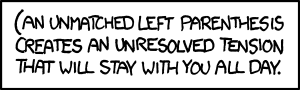
\includegraphics[scale=1.0]{(.png}\\\vspace{1\baselineskip}
<<\verb|Brains aside, I wonder how many poorly-written|\\
\verb|xkcd.com-parsing scripts will break on this title|\\
\verb|(or \;;";\''{<<;[' this mouseover text.";|>>
\end{frame}
\end{document}
